
\documentclass{beamer}


\usepackage[T1]{fontenc}
\usepackage[utf8]{inputenc}
\usepackage[english]{babel}
\usepackage{lmodern}
% \usepackage{forloop}
\usepackage{multicol}
\usepackage{animate}
\usepackage{default}
\usepackage{listing}

\usepackage[list=true]{subcaption}
\captionsetup{compatibility=false}
\usepackage{etex}


\usepackage{tikz}
\usepackage{pgfplots}

\usepackage{soul}


% \usepackage{polyglossia}
% \usepackage{listings}
% \usepackage{ulem}
% \usepackage{multicol}

% \setbeamertemplate{navigation symbols}{}
% \setbeamertemplate{sidebar right}{}
% \setbeamertemplate{footline}{\hfill\insertframenumber{} | \inserttotalframenumber}


% \newcommand{\myline}{\par
%     \kern0.5pt
%     \hrule height 0.8pt
%     \kern0.5pt
% }

\usecolortheme{cormorant}
\useoutertheme{infolines}

\definecolor{GreenHack}{RGB}{86,128, 24}

\newcommand{\hlc}[2][yellow]{ {\sethlcolor{#1} \hl{#2}} }

\title[Intro à la crypto (partie 2)]{Cryptologie}
\subtitle{Introduction à la cryptographie --- partie 2}
\author[H4ck1nTN]{Jean-Philippe Eisenbarth}
\institute[HiT]{H4ck 1n TN}
\date{\today}
\logo{
\includegraphics[width=1.3cm]{figures/logo.png}}

\begin{document}

    \begin{frame}
        \titlepage
    \end{frame}

    \frame{\tableofcontents}

    \section[Pourquoi utiliser la crypto aujourd'hui ?]{Pourquoi utiliser la crypto aujourd'hui ?}

        \begin{frame}
            Souhait de toujours plus remplacer des services traditionnels par l'informatique.

            \begin{itemize}
                \item Communication
                \item Vote
                \item Notion de confiance
            \end{itemize}

        \end{frame}

        \begin{frame}

            \begin{itemize}
                \item Confidentialité \\ \begin{center} \hlc[GreenHack]{Chiffrement} \end{center}
                \item Authenticité \\ \begin{center} \hlc[GreenHack]{Signature} \end{center}
                \item Intégrité \\ \begin{center} \hlc[GreenHack]{Hachage} \end{center}
            \end{itemize}

        \end{frame}

    \section[Cryptographie symétrique]{Cryptographie symétrique}

    \begin{frame}
        \begin{itemize}
            \item Cryptographie symétrique ou cryptographie à clé secrète.
            \item Plus ancienne ancienne forme de chiffrement.
            \item Chiffrement et déchiffrement avec la même clé. \\~\\
        \end{itemize}

        \begin{center} 2 types : chiffrement par flot, chiffrement à bloc \end{center}
    \end{frame}

    \subsection{Chiffrement par flot}

    \begin{frame}
        Chiffrement de Vernam, ou One Time Pad, ou Masque Jetable :

        \begin{itemize}
            \item le message est une suite de caractère (normal me direz vous ...)
            \item la clé doit également être une suite de caractère au moins aussi longue que le message
            \item on calcule un XOR bit à bit.
        \end{itemize}

        On obtient ainsi une suite de bit qui correspond au chiffré. \\~\\

        Pour déchiffrer on effectue un XOR entre les bits chiffrés et la clé (celle utilisée pour chiffrer)

        On jette ensuite la clé (d'où le nom One Time Pad). \\~\\

        Toute l'astuce vient du caractère aléatoire de la clé.

    \end{frame}

    \subsection{Chiffrement à bloc}

    \begin{frame}
        La différence avec le chiffrement à flot (où l'on chiffre tout d'un coup) est que l'on chiffre par bloc. \\~\\

        Exemple : DES, AES, BlowFish \\~\\

        On peut transformer un chiffrement à bloc en chiffrement par flot en utilisant un mode d'opération spécifique.
    \end{frame}

    \begin{frame}
    \frametitle{Réseau de Feistel}

    \begin{center} 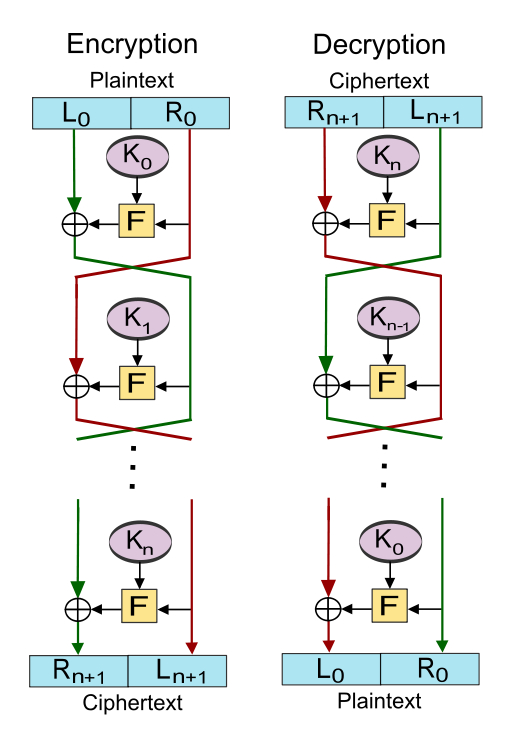
\includegraphics[scale=0.33]{figures/feistel.jpg} \end{center}

    \end{frame}

    \subsubsection{AES}

    \begin{frame}
        \begin{itemize}
            \item Taille de bloc de 128 bits
            \item Taille de clé de 128, 192 ou 256 bits
            \item Seul le bruteforce peut en venir à bout (en des temps non raisonnables)
        \end{itemize}
    \end{frame}

    \begin{frame}
    \frametitle{Réseau de substitution-permutation}

    \begin{center} 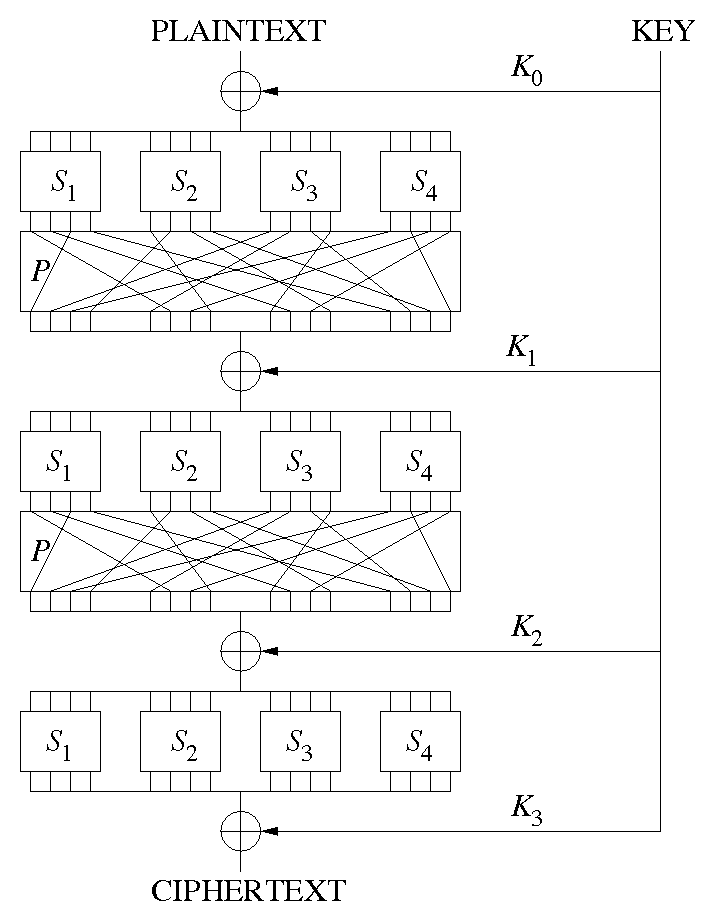
\includegraphics[scale=0.30]{figures/substitutionpermutationnetwork.png} \end{center}

    \end{frame}

    \subsubsection{Mode Op : CBC}

    \begin{frame}
        \frametitle{Mode opératoire CBC (pour le challenge ;)}

        \begin{center} 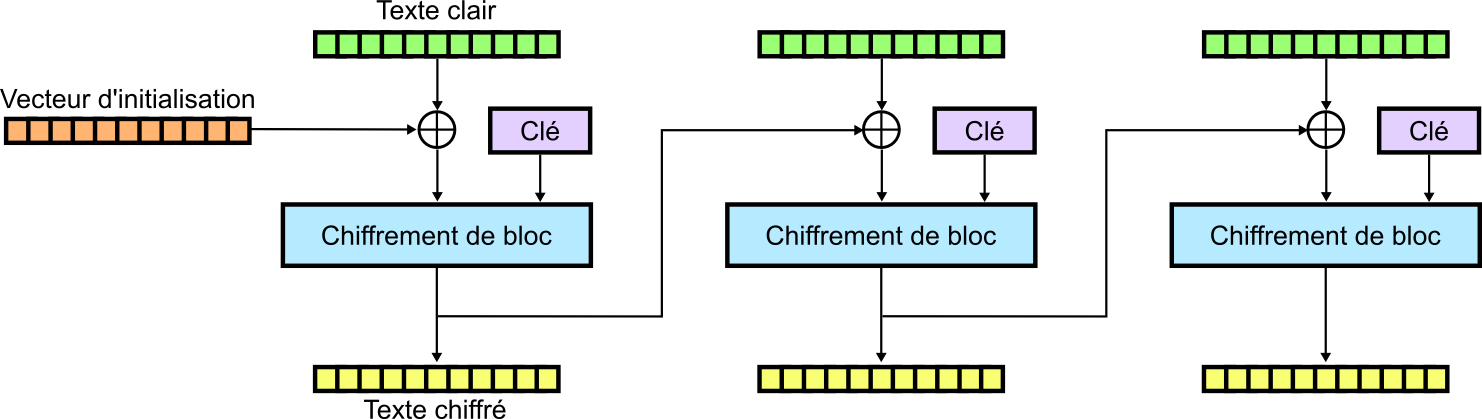
\includegraphics[scale=0.23]{figures/schema_cbc.jpg} \end{center}

    \end{frame}

    \section[Cryptographie asymétrique]{Cryptographie asymétrique}

    \begin{frame}
        \frametitle{Cryptographie à clé publique}

        Chaque personne génère un couple <clé publique>, <clé privée> \\~\\

        Envoyer un message chiffré :

        \begin{itemize}
            \item Alice utilise la clé publique de Bob pour chiffrer un message pour lui
            \item Bob utlise sa clé privée pour déchiffrer le message
        \end{itemize}

        Signer un message :
        \begin{itemize}
            \item Alice utilise sa clé privée pour signer un message pour que Bob soit sûr que c'est bien Alice qui lui parle
            \item Bob utilise la clé publique d'Alice pour vérifier que c'est bien Alice qui a envoyé le message
        \end{itemize}
    \end{frame}

    \begin{frame}
        \frametitle{Sources}
        Cours de M. Emmanuel Thomé (Cryptologie en 2A et Computer Security en 3A)
    \end{frame}

\end{document}
